\documentclass[twoside]{book}

% Packages required by doxygen
\usepackage{fixltx2e}
\usepackage{calc}
\usepackage{doxygen}
\usepackage[export]{adjustbox} % also loads graphicx
\usepackage{graphicx}
\usepackage[utf8]{inputenc}
\usepackage{makeidx}
\usepackage{multicol}
\usepackage{multirow}
\PassOptionsToPackage{warn}{textcomp}
\usepackage{textcomp}
\usepackage[nointegrals]{wasysym}
\usepackage[table]{xcolor}

% Font selection
\usepackage[T1]{fontenc}
\usepackage[scaled=.90]{helvet}
\usepackage{courier}
\usepackage{amssymb}
\usepackage{sectsty}
\renewcommand{\familydefault}{\sfdefault}
\allsectionsfont{%
  \fontseries{bc}\selectfont%
  \color{darkgray}%
}
\renewcommand{\DoxyLabelFont}{%
  \fontseries{bc}\selectfont%
  \color{darkgray}%
}
\newcommand{\+}{\discretionary{\mbox{\scriptsize$\hookleftarrow$}}{}{}}

% Page & text layout
\usepackage{geometry}
\geometry{%
  a4paper,%
  top=2.5cm,%
  bottom=2.5cm,%
  left=2.5cm,%
  right=2.5cm%
}
\tolerance=750
\hfuzz=15pt
\hbadness=750
\setlength{\emergencystretch}{15pt}
\setlength{\parindent}{0cm}
\setlength{\parskip}{3ex plus 2ex minus 2ex}
\makeatletter
\renewcommand{\paragraph}{%
  \@startsection{paragraph}{4}{0ex}{-1.0ex}{1.0ex}{%
    \normalfont\normalsize\bfseries\SS@parafont%
  }%
}
\renewcommand{\subparagraph}{%
  \@startsection{subparagraph}{5}{0ex}{-1.0ex}{1.0ex}{%
    \normalfont\normalsize\bfseries\SS@subparafont%
  }%
}
\makeatother

% Headers & footers
\usepackage{fancyhdr}
\pagestyle{fancyplain}
\fancyhead[LE]{\fancyplain{}{\bfseries\thepage}}
\fancyhead[CE]{\fancyplain{}{}}
\fancyhead[RE]{\fancyplain{}{\bfseries\leftmark}}
\fancyhead[LO]{\fancyplain{}{\bfseries\rightmark}}
\fancyhead[CO]{\fancyplain{}{}}
\fancyhead[RO]{\fancyplain{}{\bfseries\thepage}}
\fancyfoot[LE]{\fancyplain{}{}}
\fancyfoot[CE]{\fancyplain{}{}}
\fancyfoot[RE]{\fancyplain{}{\bfseries\scriptsize Generated by Doxygen }}
\fancyfoot[LO]{\fancyplain{}{\bfseries\scriptsize Generated by Doxygen }}
\fancyfoot[CO]{\fancyplain{}{}}
\fancyfoot[RO]{\fancyplain{}{}}
\renewcommand{\footrulewidth}{0.4pt}
\renewcommand{\chaptermark}[1]{%
  \markboth{#1}{}%
}
\renewcommand{\sectionmark}[1]{%
  \markright{\thesection\ #1}%
}

% Indices & bibliography
\usepackage{natbib}
\usepackage[titles]{tocloft}
\setcounter{tocdepth}{3}
\setcounter{secnumdepth}{5}
\makeindex

% Hyperlinks (required, but should be loaded last)
\usepackage{ifpdf}
\ifpdf
  \usepackage[pdftex,pagebackref=true]{hyperref}
\else
  \usepackage[ps2pdf,pagebackref=true]{hyperref}
\fi
\hypersetup{%
  colorlinks=true,%
  linkcolor=blue,%
  citecolor=blue,%
  unicode%
}

% Custom commands
\newcommand{\clearemptydoublepage}{%
  \newpage{\pagestyle{empty}\cleardoublepage}%
}

\usepackage{caption}
\captionsetup{labelsep=space,justification=centering,font={bf},singlelinecheck=off,skip=4pt,position=top}

%===== C O N T E N T S =====

\begin{document}

% Titlepage & ToC
\hypersetup{pageanchor=false,
             bookmarksnumbered=true,
             pdfencoding=unicode
            }
\pagenumbering{roman}
\begin{titlepage}
\vspace*{7cm}
\begin{center}%
{\Large My Project }\\
\vspace*{1cm}
{\large Generated by Doxygen 1.8.11}\\
\end{center}
\end{titlepage}
\clearemptydoublepage
\tableofcontents
\clearemptydoublepage
\pagenumbering{arabic}
\hypersetup{pageanchor=true}

%--- Begin generated contents ---
\chapter{File Index}
\section{File List}
Here is a list of all files with brief descriptions\+:\begin{DoxyCompactList}
\item\contentsline{section}{\hyperlink{Lab1_8c}{Lab1.\+c} }{\pageref{Lab1_8c}}{}
\end{DoxyCompactList}

\chapter{File Documentation}
\hypertarget{Matrix_8cpp}{}\section{Matrix.\+cpp File Reference}
\label{Matrix_8cpp}\index{Matrix.\+cpp@{Matrix.\+cpp}}
{\ttfamily \#include $<$iostream$>$}\\*
{\ttfamily \#include $<$cmath$>$}\\*
Include dependency graph for Matrix.\+cpp\+:
\nopagebreak
\begin{figure}[H]
\begin{center}
\leavevmode
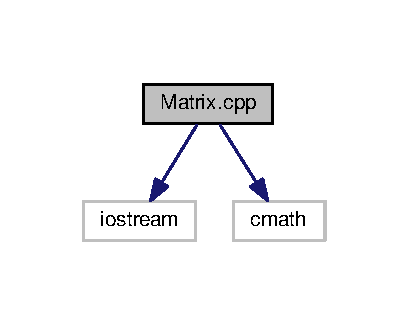
\includegraphics[width=196pt]{Matrix_8cpp__incl}
\end{center}
\end{figure}
\subsection*{Functions}
\begin{DoxyCompactItemize}
\item 
void \hyperlink{Matrix_8cpp_acd3b2475523638cdce738c5da317d699}{swapcol} (int a\mbox{[}50\mbox{]}\mbox{[}50\mbox{]}, int r, int c, int b)
\item 
void \hyperlink{Matrix_8cpp_a5a3586e1cebeb518fcc42ea59bf132aa}{swaprow} (int a\mbox{[}50\mbox{]}\mbox{[}50\mbox{]}, int r, int c, int b)
\item 
int \hyperlink{Matrix_8cpp_af95a7c0be4750d6fa2ed2db0285db104}{swapmx} (int arr\mbox{[}50\mbox{]}\mbox{[}50\mbox{]}, int m, int n, int a, int b)
\item 
void \hyperlink{Matrix_8cpp_a48e9016c0e80b5fbba89dc0d7bd319e0}{arrey} (int arr1\mbox{[}50\mbox{]}\mbox{[}50\mbox{]}, int arr2\mbox{[}50\mbox{]}\mbox{[}50\mbox{]}, int sizemx1, int p, int q)
\item 
int \hyperlink{Matrix_8cpp_ae66f6b31b5ad750f1fe042a706a4e3d4}{main} ()
\end{DoxyCompactItemize}


\subsection{Function Documentation}
\index{Matrix.\+cpp@{Matrix.\+cpp}!arrey@{arrey}}
\index{arrey@{arrey}!Matrix.\+cpp@{Matrix.\+cpp}}
\subsubsection[{\texorpdfstring{arrey(int arr1[50][50], int arr2[50][50], int sizemx1, int p, int q)}{arrey(int arr1[50][50], int arr2[50][50], int sizemx1, int p, int q)}}]{\setlength{\rightskip}{0pt plus 5cm}void arrey (
\begin{DoxyParamCaption}
\item[{int}]{arr1\mbox{[}50\mbox{]}\mbox{[}50\mbox{]}, }
\item[{int}]{arr2\mbox{[}50\mbox{]}\mbox{[}50\mbox{]}, }
\item[{int}]{sizemx1, }
\item[{int}]{p, }
\item[{int}]{q}
\end{DoxyParamCaption}
)}\hypertarget{Matrix_8cpp_a48e9016c0e80b5fbba89dc0d7bd319e0}{}\label{Matrix_8cpp_a48e9016c0e80b5fbba89dc0d7bd319e0}

\begin{DoxyCode}
319 \{
320  
321   cout<<\textcolor{stringliteral}{"Enter the elements in the 1st Array"}<<endl;
322   \textcolor{keywordflow}{for}(\textcolor{keywordtype}{int} i=0;i<sizemx1;i++)
323   \{
324     \textcolor{keywordflow}{for}(\textcolor{keywordtype}{int} j=0;j<sizemx1;j++)
325     \{
326       \textcolor{comment}{//cin>>arr1[i][j];}
327       \textcolor{keywordflow}{while}(!(cin>>arr1[i][j]))  \textcolor{comment}{//Reciving vaiables from input : is it no/character ?}
328       \{
329         cout << \textcolor{stringliteral}{"Please  enter a number!  Try again: "};
330         cin.clear ();
331         cin.ignore (1000, \textcolor{charliteral}{'\(\backslash\)n'});  \textcolor{comment}{// Skip to next newline or 1000 chars,}
332         \textcolor{comment}{// whichever comes first.}
333       \}
334  
335     \}
336   \}
337   cout<<\textcolor{stringliteral}{"Enter the elements in the 2nd Array"}<<endl;
338   \textcolor{keywordflow}{for}(\textcolor{keywordtype}{int} i=0;i<p;i++)
339   \{
340     \textcolor{keywordflow}{for}(\textcolor{keywordtype}{int} j=0;j<q;j++)
341     \{
342       \textcolor{comment}{//cin>>arr2[i][j];}
343       \textcolor{keywordflow}{while}(!(cin>>arr2[i][j]))  \textcolor{comment}{//Reciving vaiables from input : is it no/character ?}
344       \{
345         cout << \textcolor{stringliteral}{"Please  enter a number!  Try again: "};
346         cin.clear ();
347         cin.ignore (1000, \textcolor{charliteral}{'\(\backslash\)n'});  \textcolor{comment}{// Skip to next newline or 1000 chars,}
348         \textcolor{comment}{// whichever comes first.}
349       \}
350     \}
351   \}
352 \}
\end{DoxyCode}
\index{Matrix.\+cpp@{Matrix.\+cpp}!main@{main}}
\index{main@{main}!Matrix.\+cpp@{Matrix.\+cpp}}
\subsubsection[{\texorpdfstring{main()}{main()}}]{\setlength{\rightskip}{0pt plus 5cm}int main (
\begin{DoxyParamCaption}
{}
\end{DoxyParamCaption}
)}\hypertarget{Matrix_8cpp_ae66f6b31b5ad750f1fe042a706a4e3d4}{}\label{Matrix_8cpp_ae66f6b31b5ad750f1fe042a706a4e3d4}

\begin{DoxyCode}
19 \{
20   \textcolor{comment}{//-------defining variables and initializing them-------------}
21   \textcolor{keywordtype}{int} e,flag=0,i,j,flag1=0;
22   \textcolor{keywordtype}{int} arrey1[50][50],arrey2[50][50],arrey3[50][50],arrey4[50][50],arrey5[50][50],arrey6[50][50],arrey7[50][
      50],arrey8[50][50];
23   \textcolor{keywordtype}{int} k,sizemx1,p,q,r,x,y,temp=0;
24   \textcolor{keywordtype}{int} m, n,a,b,l;
25   \textcolor{keywordtype}{char} operation,redo;
26   \textcolor{comment}{//--------Printing my name on screen----------------}
27   cout<<\textcolor{stringliteral}{"Welcome to the  program 2.1 written by Your Name"}<<endl;
28   cout<<\textcolor{stringliteral}{"***************************************************************"}<<endl;
29   cout<<endl<<endl<<endl;
30  
31   cout<<\textcolor{stringliteral}{"The instruction menu:"}<<endl<<endl<<endl;
32   cout<<\textcolor{stringliteral}{"    1. Initialize Matrices"}<<endl;
33   cout<<\textcolor{stringliteral}{"    2. Print Matrices"}<<endl;
34   cout<<\textcolor{stringliteral}{"    3. Multiply Matrices"}<<endl;
35   cout<<\textcolor{stringliteral}{"    4. Transpose of 2nd Matrix"}<<endl;
36   cout<<\textcolor{stringliteral}{"    5. Move Row and Column of 2nd Matrix"}<<endl;
37   cout<<\textcolor{stringliteral}{"    6. Quit"}<<endl<<endl;
38  
39   \textcolor{comment}{//--here do loop is used so that the program can be used more then one time}
40   \textcolor{comment}{//without exiting the run screen---------------------------}
41   \textcolor{keywordflow}{do}
42   \{
43     \textcolor{keywordflow}{do}
44     \{
45  
46  
47       cout<<\textcolor{stringliteral}{"Please enter your requested instruction (1..6)?=  "};
48       \textcolor{keywordflow}{while}(!(cin>>operation))  \textcolor{comment}{//Reciving vaiables from input : is it no/character ?}
49       \{
50         cout << \textcolor{stringliteral}{"Please  enter a number!  Try again: "};
51         cin.clear ();
52         cin.ignore (1000, \textcolor{charliteral}{'\(\backslash\)n'});  \textcolor{comment}{// Skip to next newline or 1000 chars,}
53         \textcolor{comment}{// whichever comes first.}
54       \}
55       \textcolor{comment}{//cin>>operation ;}
56       cout<<endl;
57  
58  
59  
60  
61       \textcolor{comment}{//---used switch function so thet the operater can be decided------------}
62       \textcolor{keywordflow}{switch} (operation)
63       \{
64       \textcolor{comment}{//------calculating the requested equation for inputs-------------}
65       \textcolor{comment}{//-------at the same time printing the results on screen-----------}
66       \textcolor{keywordflow}{case}\textcolor{charliteral}{'1'}:
67         cout<<\textcolor{stringliteral}{"Enter the Size of 1st square Matrix"}<<endl;
68         cout<<\textcolor{stringliteral}{"Row & Column="};
69         \textcolor{keywordflow}{while}(!(cin>>sizemx1))  \textcolor{comment}{//Reciving vaiables from input : is it no/character ?}
70         \{
71           cout << \textcolor{stringliteral}{"Please  enter a number!  Try again: "};
72           cin.clear ();
73           cin.ignore (1000, \textcolor{charliteral}{'\(\backslash\)n'});  \textcolor{comment}{// Skip to next newline or 1000 chars,}
74           \textcolor{comment}{// whichever comes first.}
75         \}
76         \textcolor{comment}{//cin>>sizemx1;}
77         \textcolor{keywordflow}{if} (\textcolor{keyword}{sizeof}(sizemx1)<4)\{
78           cout<<\textcolor{stringliteral}{"unknown command"}<<endl;
79         \}
80         cout<<\textcolor{stringliteral}{"Enter the  of 2nd Matrix"}<<endl;
81         cout<<\textcolor{stringliteral}{"Row="};
82         \textcolor{keywordflow}{while}(!(cin>>p))  \textcolor{comment}{//Reciving vaiables from input : is it no/character ?}
83         \{
84           cout << \textcolor{stringliteral}{"Please  enter a number!  Try again: "};
85           cin.clear ();
86           cin.ignore (1000, \textcolor{charliteral}{'\(\backslash\)n'});  \textcolor{comment}{// Skip to next newline or 1000 chars,}
87           \textcolor{comment}{// whichever comes first.}
88         \}
89  
90         \textcolor{comment}{//cin>>p;}
91  
92         cout<<\textcolor{stringliteral}{"Column="};
93         \textcolor{keywordflow}{while}(!(cin>>q))  \textcolor{comment}{//Reciving vaiables from input : is it no/character ?}
94         \{
95           cout << \textcolor{stringliteral}{"Please  enter a number!  Try again: "};
96           cin.clear ();
97           cin.ignore (1000, \textcolor{charliteral}{'\(\backslash\)n'});  \textcolor{comment}{// Skip to next newline or 1000 chars,}
98           \textcolor{comment}{// whichever comes first.}
99         \}
100         \textcolor{comment}{//cin>>q;}
101         flag=flag+1;
102         \textcolor{comment}{//cout<<"flag="<<flag<<endl;}
103  
104  
105         \textcolor{keywordflow}{break};
106       \textcolor{keywordflow}{case}\textcolor{charliteral}{'2'}: \textcolor{comment}{//2. Print Matrices}
107         \textcolor{comment}{//cout<<"flag="<<flag<<endl;}
108         \textcolor{comment}{//cout<<"flag1="<<flag1<<endl;}
109  
110         \textcolor{keywordflow}{if}(flag<1)\{
111           cout<<\textcolor{stringliteral}{"flag="}<<flag<<endl;
112           cout<<\textcolor{stringliteral}{"Please perforform operation no.1 firest"}<<endl;
113         \}
114         \textcolor{keywordflow}{if}(flag>=1)\{
115           cout<<\textcolor{stringliteral}{"flag="}<<flag<<endl;
116           \textcolor{comment}{// arrey( arrey1,arrey2, sizemx1, p,q);}
117           \textcolor{comment}{/*cout<<"Enter the elements in the 1st Array"<<endl;}
118 \textcolor{comment}{for(i=0;i<sizemx1;i++)}
119 \textcolor{comment}{\{}
120 \textcolor{comment}{for(j=0;j<sizemx1;j++)}
121 \textcolor{comment}{\{}
122 \textcolor{comment}{cin>>arrey1[i][j];}
123 \textcolor{comment}{\}}
124 \textcolor{comment}{\}}
125 \textcolor{comment}{cout<<"Enter the elements in the 2nd Array"<<endl;}
126 \textcolor{comment}{for(i=0;i<p;i++)}
127 \textcolor{comment}{\{}
128 \textcolor{comment}{for(j=0;j<q;j++)}
129 \textcolor{comment}{\{}
130 \textcolor{comment}{cin>>arrey2[i][j];}
131 \textcolor{comment}{\}}
132 \textcolor{comment}{\}*/}
133  
134  
135  
136  
137           cout<<\textcolor{stringliteral}{"\(\backslash\)nDisplaying the 1st Array"}<<endl;
138           \textcolor{keywordflow}{for}(i=0;i<sizemx1;i++)
139           \{
140             \textcolor{keywordflow}{for}(j=0;j<sizemx1;j++)
141             \{
142               arrey1[i][j] = 50+rand() %(100-50+1);
143  
144               cout<<arrey1[i][j]<<\textcolor{stringliteral}{"\(\backslash\)t"};
145  
146             \}
147             cout<<endl;
148           \}
149           cout<<\textcolor{stringliteral}{"\(\backslash\)nDisplaying the 2nd Array"}<<endl;
150           \textcolor{keywordflow}{for}(i=0;i<p;i++)
151           \{
152             \textcolor{keywordflow}{for}(j=0;j<q;j++)
153             \{
154               arrey2[i][j] = 50+rand() %(100-50+1);
155  
156               cout<<arrey2[i][j]<<\textcolor{stringliteral}{"\(\backslash\)t"};
157             \}
158             cout<<endl;
159           \}
160           flag1=flag1+1;
161         \}
162         arrey2[10][10]=arrey4[10][10];
163  
164         \textcolor{keywordflow}{for}(i=0;i<p;i++)
165         \{
166           \textcolor{keywordflow}{for}(j=0;j<q;j++)
167           \{
168             arrey5[i][j]=arrey2[i][j];
169             arrey6[i][j]=arrey2[i][j];
170           \}
171         \}
172  
173         \textcolor{keywordflow}{break};
174       \textcolor{keywordflow}{case}\textcolor{charliteral}{'3'}:      \textcolor{comment}{//3. Multiply Matrices}
175         \textcolor{comment}{//cout<<"flag1="<<flag1<<endl;}
176         \textcolor{keywordflow}{if}(flag1<1)\{
177           cout<<\textcolor{stringliteral}{"Please perforform operation no.1 and no.2 firest"}<<endl;
178         \}\textcolor{keywordflow}{else}\{
179           \textcolor{keywordflow}{if}(sizemx1!=p)\{
180             cout<<\textcolor{stringliteral}{"Multiplication is not possible"}<<endl;
181           \}
182           \textcolor{keywordflow}{if}(sizemx1==p)
183           \{
184             \textcolor{keywordflow}{for}(i=0;i<sizemx1;i++)
185             \{
186               \textcolor{keywordflow}{for}(j=0;j<q;j++)
187               \{
188                 arrey3[i][j]=0;
189                 \textcolor{keywordflow}{for}(k=0;k<p;k++)
190                 \{
191                   arrey3[i][j]=arrey3[i][j]+arrey1[i][k]*arrey2[k][j];
192                 \}
193               \}
194             \}
195             cout<<\textcolor{stringliteral}{"\(\backslash\)nDisplaying the array elements after multiplication"}<<endl;
196             \textcolor{keywordflow}{for}(i=0;i<sizemx1;i++)
197             \{
198               \textcolor{keywordflow}{for}(j=0;j<q;j++)
199               \{
200                 cout<<arrey3[i][j]<<\textcolor{stringliteral}{"\(\backslash\)t"};
201               \}
202               cout<<endl;
203             \}
204           \}
205         \}
206         \textcolor{keywordflow}{break};
207       \textcolor{keywordflow}{case}\textcolor{charliteral}{'4'}:   \textcolor{comment}{//4. Transpose of 2nd Matrix}
208  
209         \textcolor{keywordflow}{if}(flag1<1)\{
210           cout<<\textcolor{stringliteral}{"Please perforform operation no.1 and no.2 firest"}<<endl;
211         \}
212         \textcolor{keywordflow}{else}\{
213           \textcolor{keywordflow}{for}(i=0;i<p;i++)
214           \{
215             \textcolor{keywordflow}{for}(j=0;j<q;j++)
216             \{
217               arrey7[i][j]=arrey6[i][j];
218  
219             \}
220           \}
221           cout<<\textcolor{stringliteral}{"\(\backslash\)nDisplaying trannspose the 2nd Matrix"}<<endl;
222  
223           \textcolor{keywordflow}{for}(i=0;i<=q-1;i++)
224           \{
225             \textcolor{keywordflow}{for}(j=0;j<=p-1;j++)
226             \{
227               temp=arrey7[j][i];
228               arrey7[j][i]=arrey4[i][j];
229               arrey4[i][j]=temp;
230  
231               \textcolor{comment}{//cout<<i<<j;}
232               cout<<temp<<\textcolor{stringliteral}{"\(\backslash\)t"};
233             \}
234             cout<<endl;
235           \}
236         \}
237  
238         \textcolor{keywordflow}{break};
239       \textcolor{keywordflow}{case}\textcolor{charliteral}{'5'}: \textcolor{comment}{//5. Move Row and Column of 2nd Matrix}
240  
241         \textcolor{keywordflow}{if}(flag1<1)\{
242           cout<<\textcolor{stringliteral}{"Please perforform operation no.1 and no.2 firest"}<<endl;
243         \}    \textcolor{keywordflow}{else}\{
244  
245           cout <<\textcolor{stringliteral}{"enter the row number you want to swap:"}<<endl;
246           \textcolor{comment}{// cin>>x>>y;}
247  
248           \textcolor{keywordflow}{while}(!(cin>>x))  \textcolor{comment}{//Reciving vaiables from input : is it no/character ?}
249           \{
250             cout << \textcolor{stringliteral}{"Please  enter a number!  Try again: "};
251             cin.clear ();
252             cin.ignore (1000, \textcolor{charliteral}{'\(\backslash\)n'});  \textcolor{comment}{// Skip to next newline or 1000 chars,}
253             \textcolor{comment}{// whichever comes first.}
254           \}
255           cout<<endl;
256           cout <<\textcolor{stringliteral}{"enter the column number you want to swap:"}<<endl;
257           \textcolor{keywordflow}{while}(!(cin>>y))  \textcolor{comment}{//Reciving vaiables from input : is it no/character ?}
258           \{
259             cout << \textcolor{stringliteral}{"Please  enter a number!  Try again: "};
260             cin.clear ();
261             cin.ignore (1000, \textcolor{charliteral}{'\(\backslash\)n'});  \textcolor{comment}{// Skip to next newline or 1000 chars,}
262             \textcolor{comment}{// whichever comes first.}
263           \}
264           cout<<endl;
265  
266           \textcolor{keywordflow}{for}(i=0;i<p;i++)
267           \{
268             \textcolor{keywordflow}{for}(j=0;j<q;j++)
269             \{
270               arrey8[i][j]=arrey5[i][j];
271  
272             \}
273           \}
274           cout<<\textcolor{stringliteral}{"The original matrix is"}<<endl;
275           cout<< endl;
276  
277           \textcolor{keywordflow}{for}(i=0;i<p;i++)
278           \{
279             \textcolor{keywordflow}{for}(j=0;j<q;j++)
280             \{
281  
282  
283               cout<<arrey8[i][j]<<\textcolor{stringliteral}{"\(\backslash\)t"};
284             \}
285             cout<< endl;
286           \}
287  
288           \hyperlink{Matrix_8cpp_af95a7c0be4750d6fa2ed2db0285db104}{swapmx}(arrey8,p,q,x,y);
289           cout<< endl;
290  
291         \}
292         \textcolor{keywordflow}{break};
293       \textcolor{keywordflow}{case}\textcolor{charliteral}{'6'}:  \textcolor{comment}{//  6. Quit}
294         cout<<\textcolor{stringliteral}{"Thanks do u want to start again:"};
295         cout<<endl<<endl;
296         \textcolor{keywordflow}{goto} label;
297         \textcolor{keywordflow}{break};
298       \textcolor{keywordflow}{default}:
299         cout<<\textcolor{stringliteral}{"unknown command"}<<endl;
300  
301       \}
302     \}
303     \textcolor{keywordflow}{while}(operation==\textcolor{charliteral}{'1'}||operation==\textcolor{charliteral}{'2'}||operation==\textcolor{charliteral}{'3'}||operation==\textcolor{charliteral}{'4'}||operation==\textcolor{charliteral}{'5'}||operation==\textcolor{charliteral}{'6'});
304  
305  
306     \textcolor{comment}{//----now once again the program will ask the user if want to continue or not}
307     cout<<\textcolor{stringliteral}{"enter y or Y to continue:"};
308     cin>>redo;
309     cout<<endl<<endl;
310   \}
311   \textcolor{keywordflow}{while}(redo==\textcolor{charliteral}{'y'}||redo==\textcolor{charliteral}{'Y'});
312 label:
313  
314   system(\textcolor{stringliteral}{"pause"});
315   \textcolor{keywordflow}{return} 0;
316  
317 \}
\end{DoxyCode}


Here is the call graph for this function\+:
\nopagebreak
\begin{figure}[H]
\begin{center}
\leavevmode
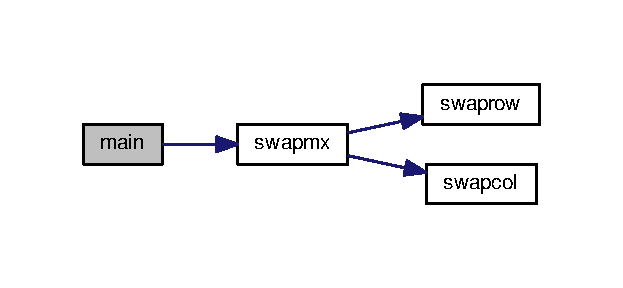
\includegraphics[width=299pt]{Matrix_8cpp_ae66f6b31b5ad750f1fe042a706a4e3d4_cgraph}
\end{center}
\end{figure}


\index{Matrix.\+cpp@{Matrix.\+cpp}!swapcol@{swapcol}}
\index{swapcol@{swapcol}!Matrix.\+cpp@{Matrix.\+cpp}}
\subsubsection[{\texorpdfstring{swapcol(int a[50][50], int r, int c, int b)}{swapcol(int a[50][50], int r, int c, int b)}}]{\setlength{\rightskip}{0pt plus 5cm}void swapcol (
\begin{DoxyParamCaption}
\item[{int}]{a\mbox{[}50\mbox{]}\mbox{[}50\mbox{]}, }
\item[{int}]{r, }
\item[{int}]{c, }
\item[{int}]{b}
\end{DoxyParamCaption}
)}\hypertarget{Matrix_8cpp_acd3b2475523638cdce738c5da317d699}{}\label{Matrix_8cpp_acd3b2475523638cdce738c5da317d699}

\begin{DoxyCode}
355 \{
356   \textcolor{keywordtype}{int} t,s;
357   \textcolor{keywordflow}{while}(b < (c-1))
358   \{
359     \textcolor{keywordflow}{for}(\textcolor{keywordtype}{int} i=0; i<r; i++)
360     \{
361       t = a[i][b];
362       a[i][b] = a[i][b+1];
363       a[i][b+1] = t;
364     \}
365     b++;
366   \}
367  
368  
369 \}
\end{DoxyCode}
\index{Matrix.\+cpp@{Matrix.\+cpp}!swapmx@{swapmx}}
\index{swapmx@{swapmx}!Matrix.\+cpp@{Matrix.\+cpp}}
\subsubsection[{\texorpdfstring{swapmx(int arr[50][50], int m, int n, int a, int b)}{swapmx(int arr[50][50], int m, int n, int a, int b)}}]{\setlength{\rightskip}{0pt plus 5cm}int swapmx (
\begin{DoxyParamCaption}
\item[{int}]{arr\mbox{[}50\mbox{]}\mbox{[}50\mbox{]}, }
\item[{int}]{m, }
\item[{int}]{n, }
\item[{int}]{a, }
\item[{int}]{b}
\end{DoxyParamCaption}
)}\hypertarget{Matrix_8cpp_af95a7c0be4750d6fa2ed2db0285db104}{}\label{Matrix_8cpp_af95a7c0be4750d6fa2ed2db0285db104}

\begin{DoxyCode}
393 \{
394  
395   \textcolor{keywordtype}{int}  i, j,k,l;
396  
397   \textcolor{comment}{//for( l = 0; l <=a-1; l ++)\{}
398   \textcolor{comment}{/* Swap function call */}
399   cout<<\textcolor{stringliteral}{"The matrix after shifting row"}<<endl;
400   \hyperlink{Matrix_8cpp_a5a3586e1cebeb518fcc42ea59bf132aa}{swaprow}(arr, m, n, a-1);
401   \textcolor{keywordflow}{for}( i = 0; i < m ; i ++)
402   \{ cout<< endl;
403     \textcolor{keywordflow}{for} (  j = 0; j < n ; j ++)
404  
405       cout << arr[i][j] <<\textcolor{stringliteral}{"\(\backslash\)t"};
406   \}
407   cout<< endl;
408   cout<< endl;
409  
410  
411   \textcolor{comment}{//\}}
412   cout<<endl<<endl;
413   cout<<\textcolor{stringliteral}{"The matrix after shifting column"}<<endl;
414   \textcolor{comment}{//for( k = 0; k <=b ; k ++)\{}
415  
416  
417   \hyperlink{Matrix_8cpp_acd3b2475523638cdce738c5da317d699}{swapcol}(arr, m, n, b-1);
418   \textcolor{comment}{//cout<<"k="<<k<<endl;}
419   \textcolor{comment}{/* Display Array in Matrix form */}
420   \textcolor{comment}{//\}}
421   \textcolor{keywordflow}{for}( i = 0; i < m ; i ++)
422   \{ cout<< endl;
423     \textcolor{keywordflow}{for} (  j = 0; j < n ; j ++)
424       cout << arr[i][j] <<\textcolor{stringliteral}{"\(\backslash\)t"};
425   \}
426   cout<< endl;
427   \textcolor{keywordflow}{return} 1;
428 \}
\end{DoxyCode}


Here is the call graph for this function\+:
\nopagebreak
\begin{figure}[H]
\begin{center}
\leavevmode
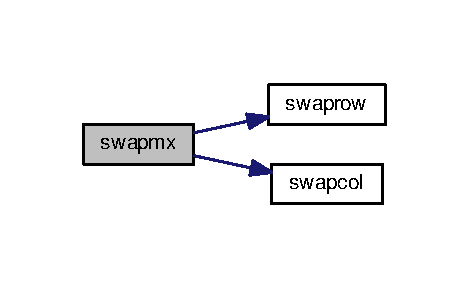
\includegraphics[width=225pt]{Matrix_8cpp_af95a7c0be4750d6fa2ed2db0285db104_cgraph}
\end{center}
\end{figure}


\index{Matrix.\+cpp@{Matrix.\+cpp}!swaprow@{swaprow}}
\index{swaprow@{swaprow}!Matrix.\+cpp@{Matrix.\+cpp}}
\subsubsection[{\texorpdfstring{swaprow(int a[50][50], int r, int c, int b)}{swaprow(int a[50][50], int r, int c, int b)}}]{\setlength{\rightskip}{0pt plus 5cm}void swaprow (
\begin{DoxyParamCaption}
\item[{int}]{a\mbox{[}50\mbox{]}\mbox{[}50\mbox{]}, }
\item[{int}]{r, }
\item[{int}]{c, }
\item[{int}]{b}
\end{DoxyParamCaption}
)}\hypertarget{Matrix_8cpp_a5a3586e1cebeb518fcc42ea59bf132aa}{}\label{Matrix_8cpp_a5a3586e1cebeb518fcc42ea59bf132aa}

\begin{DoxyCode}
372 \{
373   \textcolor{keywordtype}{int} t;
374   \textcolor{keywordflow}{while}(b < (r-1))
375   \{
376     \textcolor{keywordflow}{for}(\textcolor{keywordtype}{int} i=0; i<c; i++)
377     \{
378       t = a[b][i];
379       a[b][i] = a[b+1][i];
380       a[b+1][i] = t;
381     \}
382     b++;
383   \}
384  
385   \textcolor{comment}{/*for(int i = 0; i< c ; i++)}
386 \textcolor{comment}{\{}
387 \textcolor{comment}{t = a[b-1][i];}
388 \textcolor{comment}{a[b-1][i] = a[r-1][i];}
389 \textcolor{comment}{a[r-1][i] = t;}
390 \textcolor{comment}{\}*/}
391 \}
\end{DoxyCode}

%--- End generated contents ---

% Index
\backmatter
\newpage
\phantomsection
\clearemptydoublepage
\addcontentsline{toc}{chapter}{Index}
\printindex

\end{document}
